\section{Variables Estadísticas Unidimensionales}


\begin{ejercicio}
    El número de hijos de las familias de una determinada barriada de una ciudad es una variable estadística de la que se conocen los siguientes datos:
    \begin{equation*}
        \begin{array}{|c|c|c|c|}
            x_i & n_i & N_i & f_i \\ \hline
            0 & 80 & & 0.16 \\
            1 & 110 & & \\
            2 & & 320 & \\
            3 & & & 0.18\\
            4 & 40 & & \\
            5 & & & \\
            6 & 20 & & \\ \hline
        \end{array}
    \end{equation*}

    Sea el número de hijos de una familia, $X$, una variable estadística con población $n=500$ y modalidades $x_1, \dots, x_6$ con \emph{distribución de frecuencias}:
    $$\{x_i, n_i\}_{i=1, \dots, 7}$$
    \begin{enumerate}
        \item Completar la tabla de frecuencias.
        \begin{equation*}
            \begin{array}{|c|c|c|c|}
                x_i & n_i & N_i & f_i \\ \hline
                0 & 80 & 80 & 0.16 \\
                1 & 110 & 190 & 0.22 \\
                2 & 130 & 320 & 0.26\\
                3 & 90 & 410 & 0.18\\
                4 & 40 & 450 & 0.08\\
                5 & 30 & 480 & 0.06\\
                6 & 20 & 500 & 0.04\\ \hline
            \end{array}
        \end{equation*}

        \item Representar la distribución mediante un diagrama de barras y la curva de distribución.
        \begin{figure}[H]
            \centering
            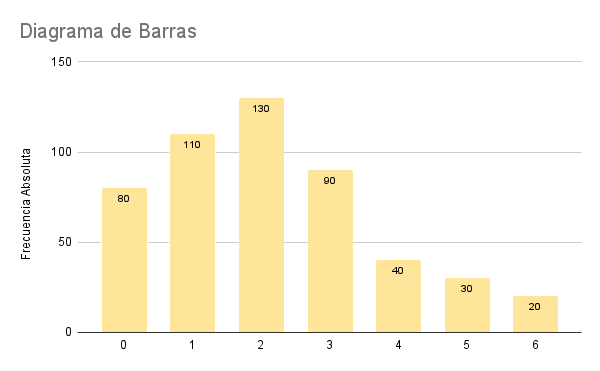
\includegraphics[width=\linewidth]{Imagenes/Barras_Ej1.png}
            \caption{Diagrama de Barras}
        \end{figure}
        \begin{figure}[H]
            \centering
            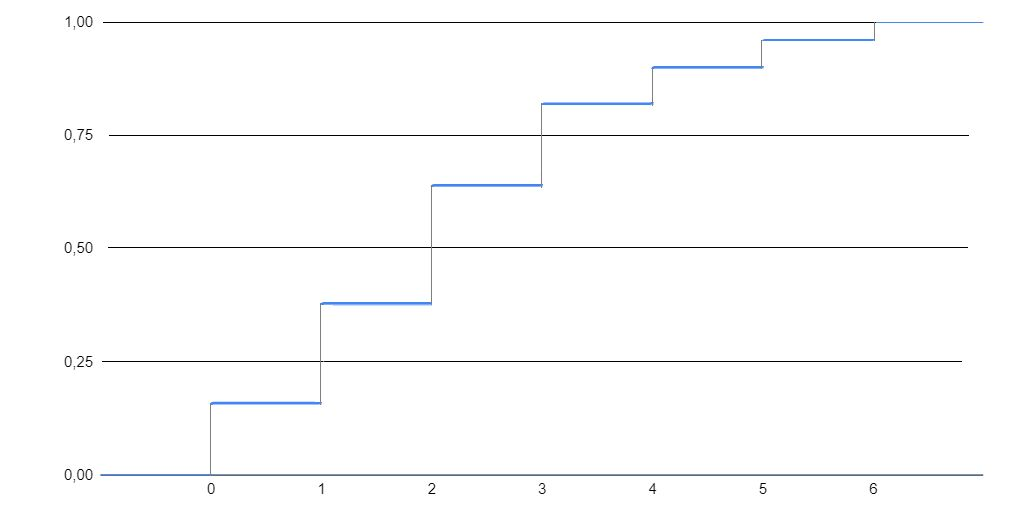
\includegraphics[width=\linewidth]{Imagenes/CDF.jpg}
            \caption{Curva de distribución}
        \end{figure}

        \item Promediar los valores de la variable mediante diferentes medidas. Interpretarlas.
        $$\bar{x} = \frac{1}{n} \sum_{i=1}^7 n_ix_i = \frac{1070}{500} = 2.14 \qquad Me=2 \qquad Mo=2$$
        La media aritmética nos informa de que en la población estudiada la media de hijos es aproximadamente 2.

        La moda nos informa de que el valor más usual, es decir, el número de hijos más repetidos, es 2.

        La mediana nos indica que más de la mitad de los encuestados tienen 2 o menos hijos.
    \end{enumerate}
\end{ejercicio}


\begin{ejercicio}
    La puntuación obtenida por 50 personas que se presentaron a una prueba de selección, sumadas las puntuaciones de los distintos tests, fueron:
    \begin{multline*}
        174,\;185,\;166,\;176,\;145,\;166,\;191,\;175,\;158,\;156,\;156,\;187,\;162,\;172,\;197,\;181,\;151,\;\\
        161,\;183,\;172,\;162,\;147,\;178,\;176,\;141,\;170,\;171,\;158,\;184,\;173,\;169,\;162,\;172,\;181,\;\\
        187,\;177,\;164,\;171,\;193,\;183,\;173,\;179,\;188,\;179,\;167,\;178,\;180,\;168,\;148,\;173.
    \end{multline*}

    \begin{enumerate}
        \item Agrupar los datos en intervalos de amplitud 5 desde 140 a 200 y dar la tabla de frecuencias.\\
        Sea la puntuación obtenida en una prueba de selección, $X$, una variable estadística continua con población $n=50$ e intervalos $I_1, \dots, I_{12}$ con \emph{distribución de frecuencias}:
        $$\{I_i, n_i\}_{i=1, \dots, 12}$$

        \begin{equation*}
            \begin{array}{|c|c|c|c|c|c|c|c|}
                 I_i  & n_i & N_i & f_i & F_i & a_i & h_i & c_i \\  \hline
                \left[140, 145\right] & 2 & 2 & 0.04 & 0.04 & 5 & 0.4  & 142.5\\
                (145, 150] & 2 & 4 & 0.04 & 0.08 & 5 & 0.4  & 147.5\\
                (150, 155] & 1 & 5 & 0.02 & 0.1  & 5 & 0.2  & 152.5\\
                (155, 160] & 4 & 9 & 0.08 & 0.18 & 5 & 0.8  & 157.5\\
                (160, 165] & 5 & 14& 0.1  & 0.28 & 5 & 1 & 162.5\\
                (165, 170] & 6 & 20& 0.12 & 0.4  & 5 & 1.2  & 167.5\\
                (170, 175] & 10& 30& 0.2  & 0.6  & 5 & 2 & 172.5\\
                (175, 180] & 8 & 38& 0.16 & 0.76 & 5 & 1.6  & 177.5\\
                (180, 185] & 6 & 44& 0.12 & 0.88 & 5 & 1.2  & 182.5\\
                (185, 190] & 3 & 47& 0.06 & 0.94 & 5 & 0.6  & 187.5\\
                (190, 195] & 2 & 49& 0.04 & 0.98 & 5 & 0.4  & 192.5\\
                (195, 200] & 1 & 50& 0.02 & 1 & 5 & 0.2  & 197.5 \\ \hline
            \end{array}
        \end{equation*}

        \item Representar la distribución mediante un histograma, poligonal de frecuencias y curva de distribución.
        \begin{figure}[H]
            \centering
            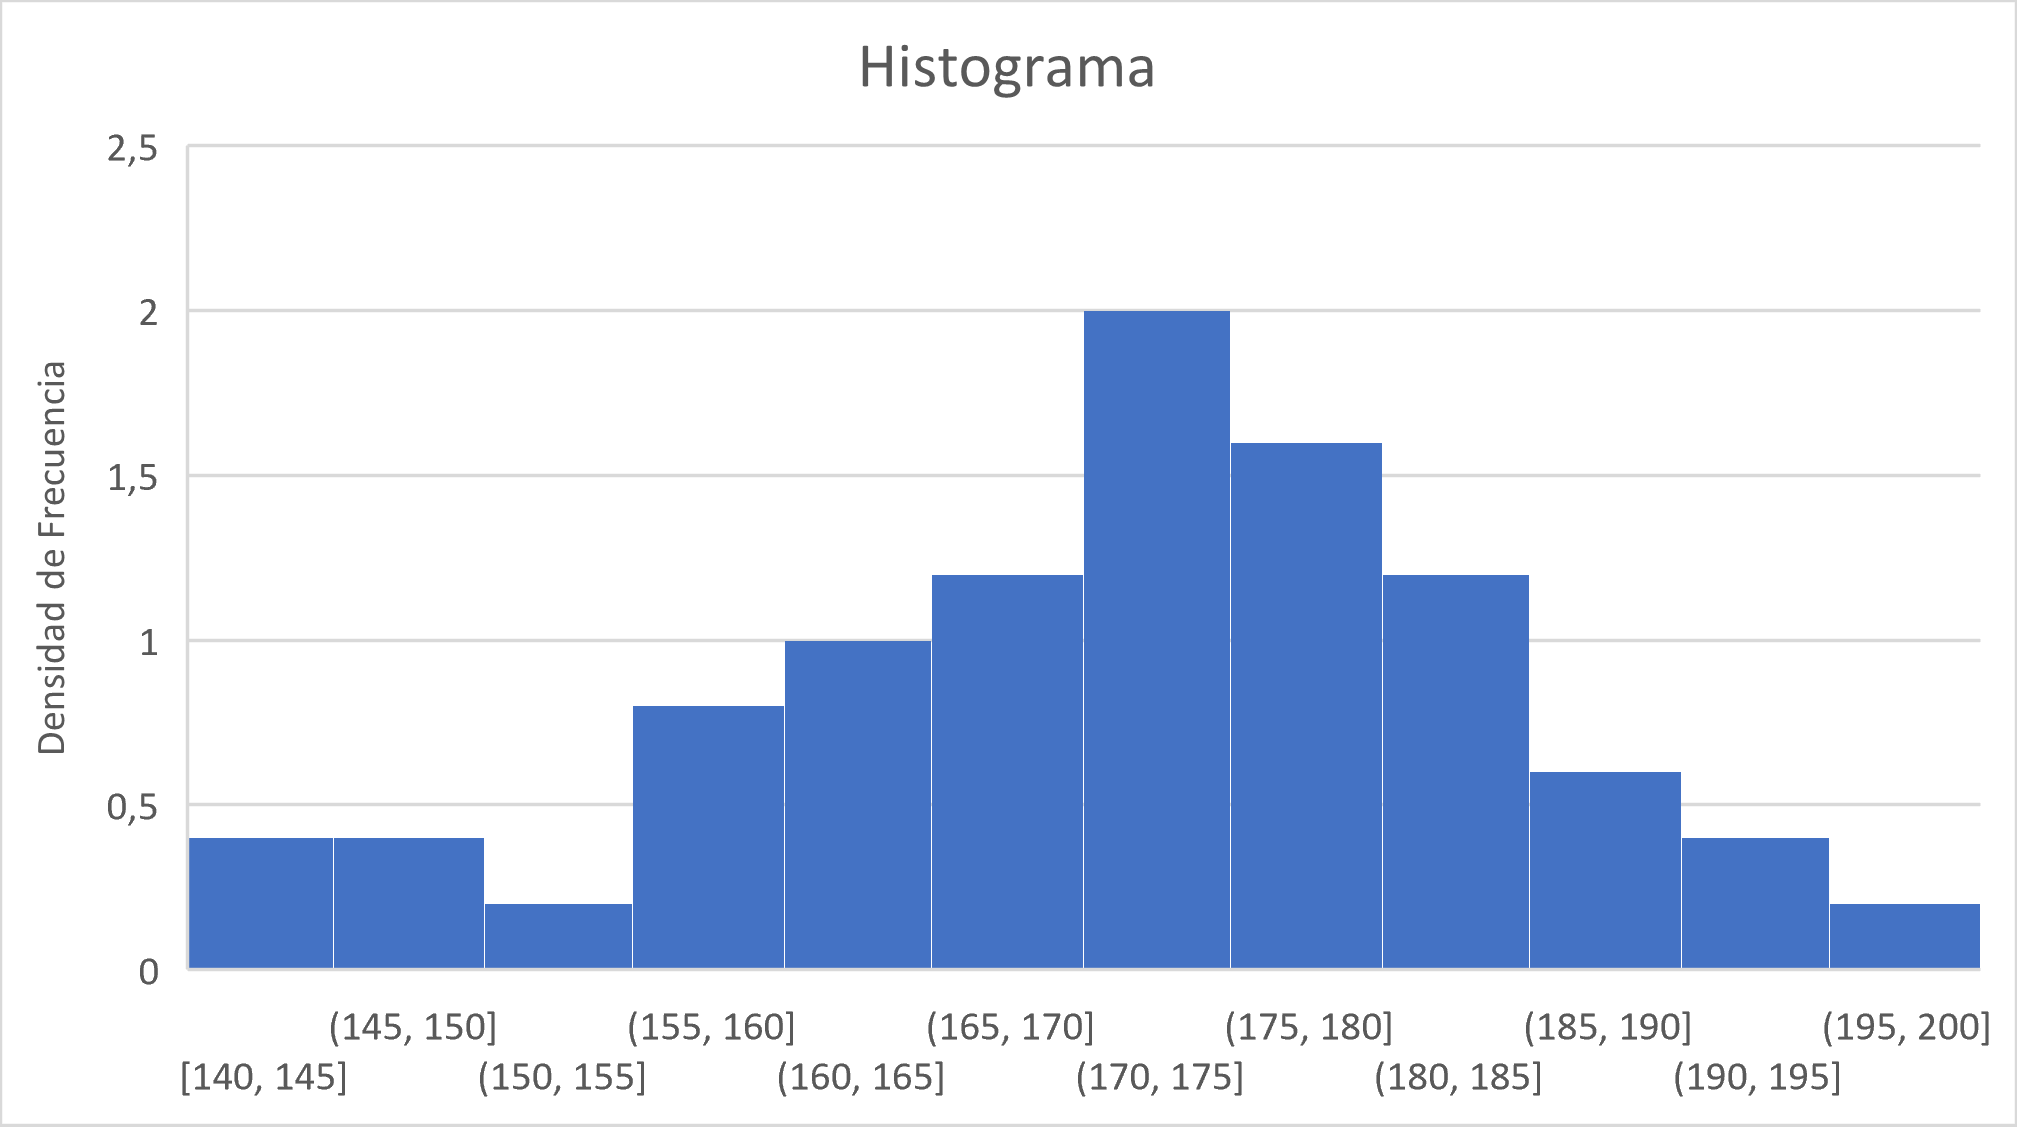
\includegraphics[width=0.7\linewidth]{Imagenes/Histograma_Ej2.png}
            \caption{Histograma}
        \end{figure}
        \begin{figure}[H]
            \centering
            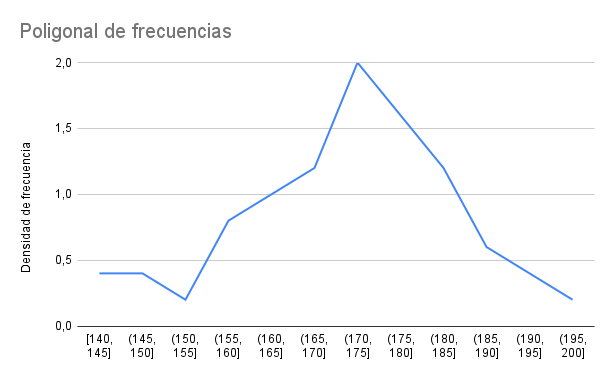
\includegraphics[width=0.7\linewidth]{Imagenes/Poligonal_frec_Ej2.png}
            \caption{Poligonal de frecuencias}
        \end{figure}
        \begin{figure}[H]
            \centering
            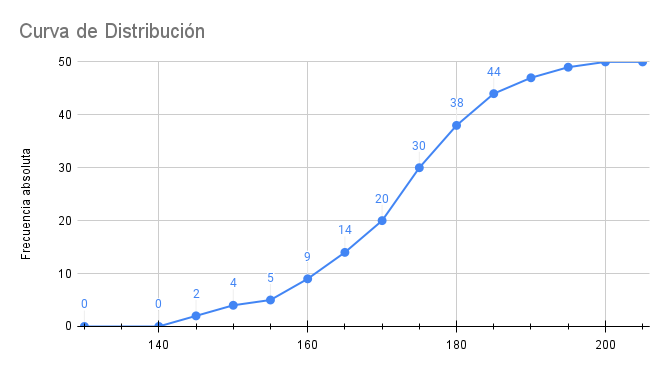
\includegraphics[width=\linewidth]{Imagenes/Curva_Ej2.png}
            \caption{Curva de distribución}
        \end{figure}
    \end{enumerate}
\end{ejercicio}

\begin{ejercicio}
    La distribución de la renta familiar en el año 2003 por comunidades autónomas se recoge en la siguiente tabla:
    \begin{equation*}
            \begin{array}{|c|c|c|c|c|c|c|c|}
                I_i & n_i & N_i & f_i & F_i & c_i& a_i & h_i \\ \hline
                (8300,\;9300]   & 2 &   &   &    &   &   & \\
                ,\;10200]  &   & 5 &   &    &  &   & \\
                 &   &  &  & 10/18  & &  & \\
                 &   &  & 2/18 &   & 12000&  &\\
                 & 4 &  &   &    &  &    & 0.005/18 \\
                 &   & 18&   &        &  &   & 0.002/18 \\ \hline
            \end{array}
        \end{equation*}
    

    \begin{enumerate}
        \item Completar la tabla.
        Sea la renta familiar en el año 2003, $X$, una variable estadística continua con población $n=18$ e intervalos $I_1, \dots, I_{6}$ con \emph{distribución de frecuencias}:
        $$\{I_i, n_i\}_{i=1, \dots, 6}$$
        \begin{equation*}
        \begin{array}{|c|c|c|c|c|c|c|c|}
            I_i & n_i & N_i & f_i & F_i & c_i& a_i & h_i \\ \hline
            (8300,\;9300]   & 2 & 2 & 2/18 & 2/18   & 8800 & 1000 & 0.002/18\\
            (9300,\;10200]  & 3 & 5 & 3/18 & 5/18   & 9750 & 900  & 0.00\bar{3}/18\\
            (10200,\;11300] & 5 & 10& 5/18 & 10/18  & 10750& 1100 & 0.00\overline{45}/18\\
            (11300,\;12700] & 2 & 12& 2/18 & 12/18  & 12000& 1400 & 0.001428/18\\
            (12700,\;13500] & 4 & 16& 4/18 & 16/18  & 13100& 800  & 0.005/18 \\
            (13500,\;14500] & 2 & 18& 2/18 & 1      & 14000& 1000 & 0.002/18 \\ \hline
        \end{array}
    \end{equation*}

        \vspace{2cm}
        \item Representar la distribución mediante un histograma, poligonal de frecuencias y curva de distribución.
        \begin{figure}[H]
            \centering
            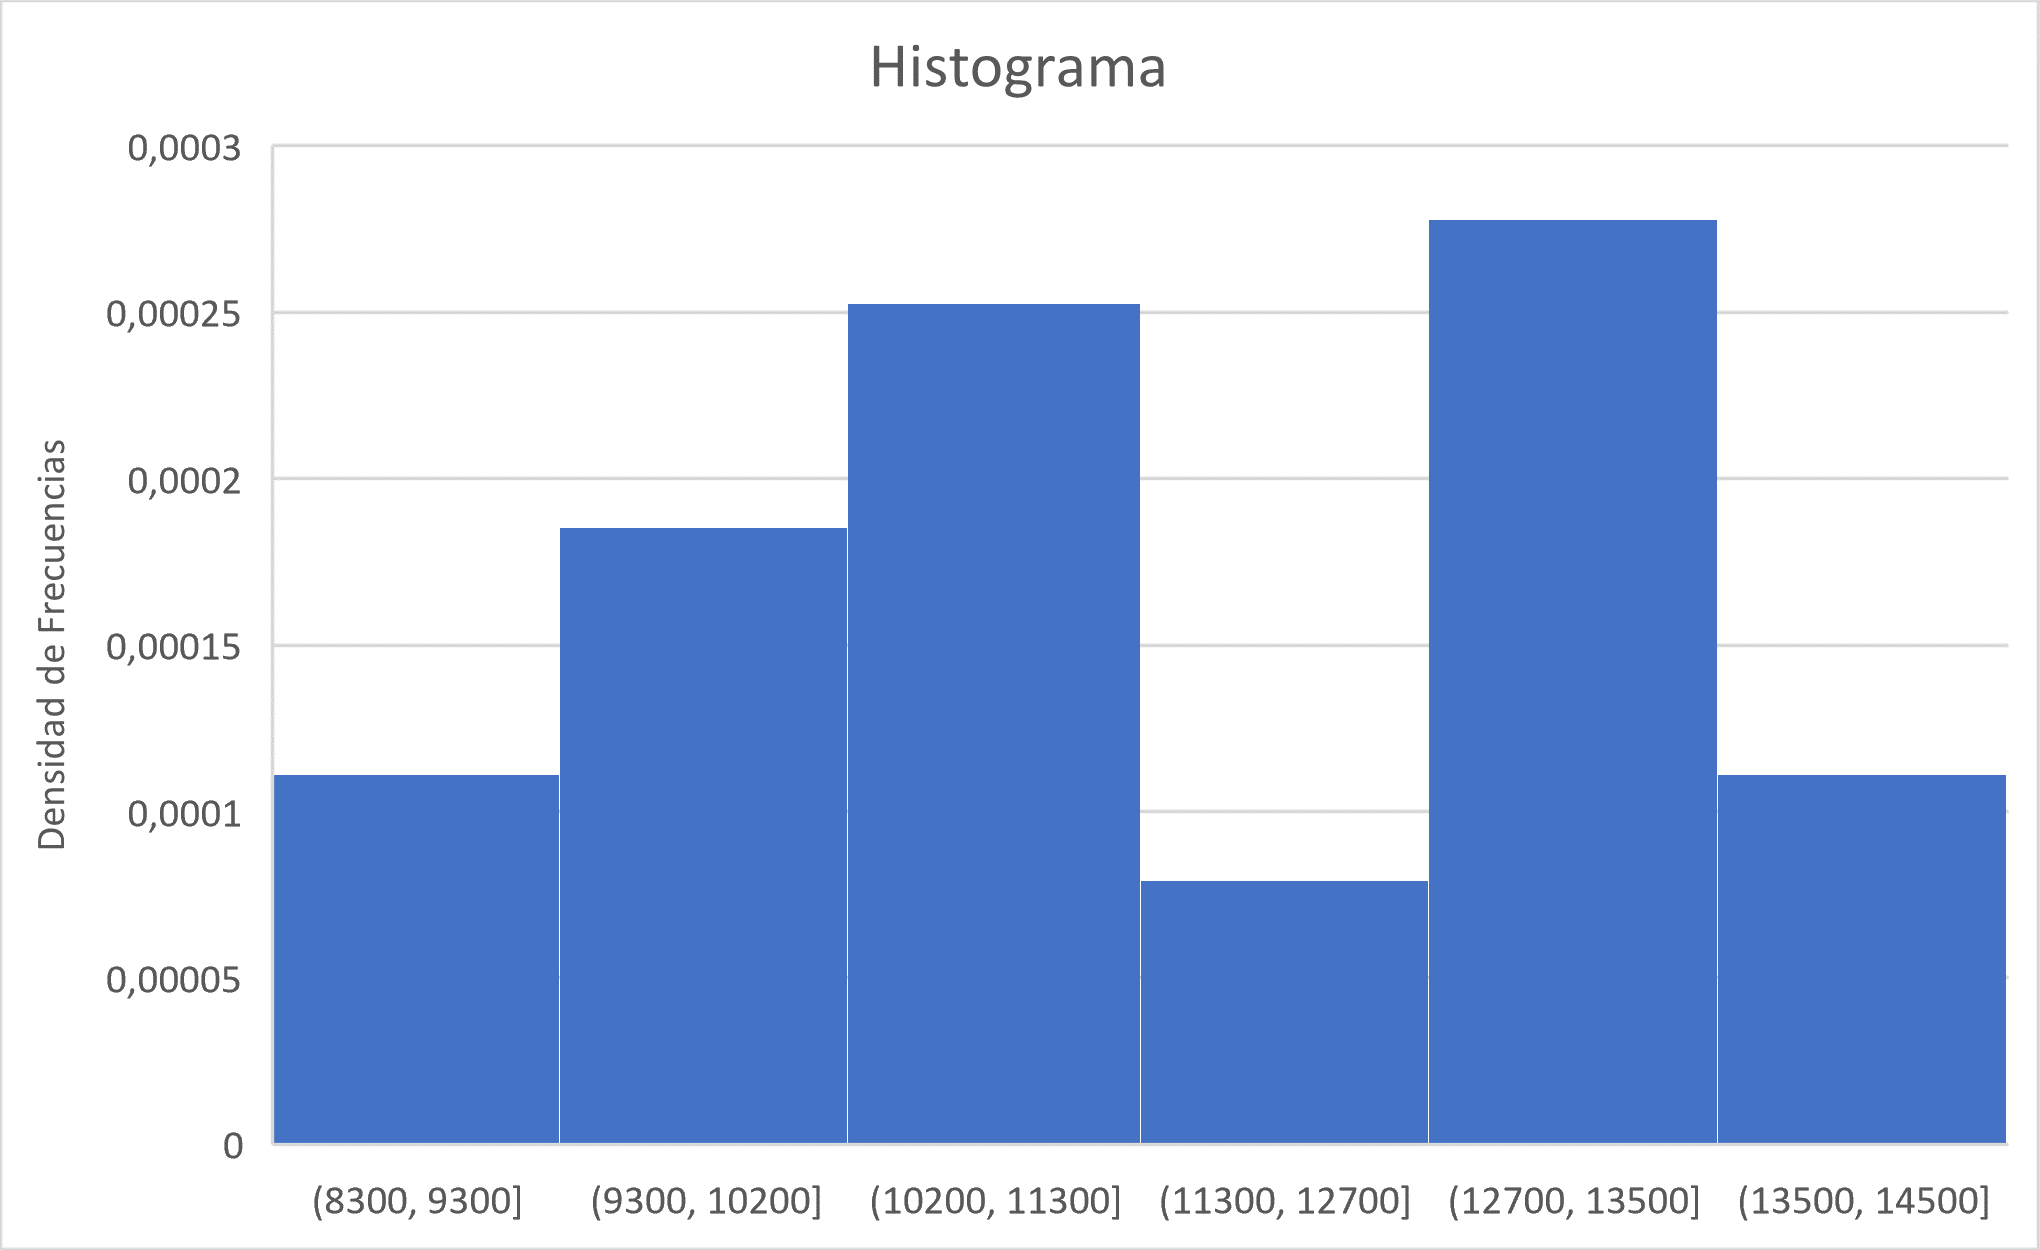
\includegraphics[width=0.6\linewidth]{Imagenes/Ej3_Histograma.png}
            \caption{Histograma}
        \end{figure}
        \begin{figure}[H]
            \centering
            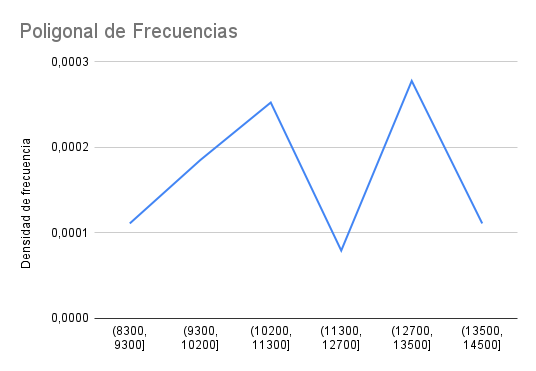
\includegraphics[width=0.6\linewidth]{Imagenes/Ej3_Poligonal.png}
            \caption{Poligonal de Frecuencias}
        \end{figure}
        \begin{figure}[H]
            \centering
            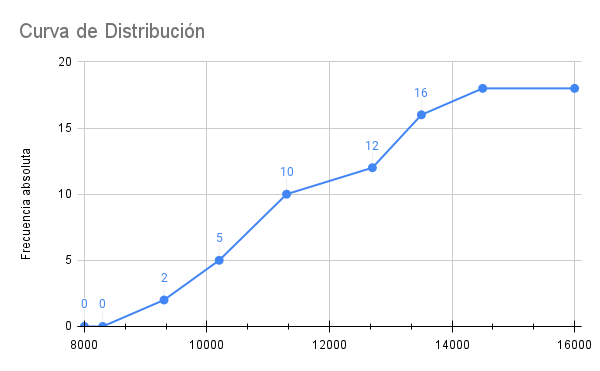
\includegraphics[width=0.7\linewidth]{Imagenes/Ej3_Distribucion.png}
            \caption{Curva de Distribución}
        \end{figure}
        
        \item ¿Cuántas comunidades presentan una renta menor o igual que $12700$ euros? ¿Y cuántas superior a $11300$ euros? 

        Observando la tabla, es fácil ver que hay $12$ comunidades autónomas cuya renta familiar es menor que $12700$ euros. Esto se debe a que $N_4=12$, y $e_4=12700$.

        Además, se puede ver que hay $8$ comunidades con renta mayor que $11300$ euros. Esto se debe a que $e_3 = 11300$ y que $n-N_3 = 18-10 = 8$.

    \end{enumerate}
\end{ejercicio}

\begin{ejercicio}
    En una determinada empresa se realiza un estudio sobre la calidad de su producción. La distribución siguiente informa sobre el número de piezas defectuosas encontradas en 100 cajas examinadas con 50 unidades cada una de ellas:
    \begin{table}[H]
        \centering
        \begin{tabular}{c||c||c|c|c|c|c|c|c|c|c|c|c|}
            \hline
            $x_i$ & N$^o$ piezas defectuosas & 0 & 1 & 2 & 3 & 4 & 5 & 6 & 7 & 8 & 9 & 10  \\ \hline
            $n_i$ & N$^o$ de cajas & 6 & 9 & 10 & 11 & 14 & 16 & 16 & 9 & 4 & 3 & 2 \\ \hline
        \end{tabular}
    \end{table}

    \begin{enumerate}
        \item Calcular el número medio de piezas defectuosas por caja.\\
        Sea el número de piezas defectuosas por caja, $X$, una variable estadística con población $n=100$ y modalidades $x_1, \dots, x_11$ con \emph{distribución de frecuencias}:
        $$\{x_i, n_i\}_{i=1, \dots, 11}$$

        La media aritmética es:
        $$\bar{x} = \frac{\sum_{i=1}^{11}n_ix_i}{\sum_{i=1}^{11}n_i} = \frac{436}{100} = 4.36 \text{ piezas defectuosas por caja.}$$

        \item ¿Cuántas piezas defectuosas se encuentran más frecuentemente en las cajas examinadas?\\
        Hay dos valores modales: $Mo=\{5,6\}$, con una frecuencia absoluta $f_i = 16$.

        \item ¿Cuál es el número mediano de piezas defectuosas por caja?
        \begin{table}[H]
            \centering
            \begin{tabular}{c||c||c|c|c|c|c|c|c|c|c|c|c|}
                \hline
                $x_i$ & N$^o$ piezas defectuosas & 0 & 1 & 2 & 3 & 4 & 5 & 6 & 7 & 8 & 9 & 10  \\ \hline
                $n_i$ & N$^o$ de cajas & 6 & 9 & 10 & 11 & 14 & 16 & 16 & 9 & 4 & 3 & 2 \\ \hline
                $N_i$ &  & 6 & 15 & 25 & 36 & 50 & 66 & 82 & 91 & 95 & 98 & 100 \\ \hline
            \end{tabular}
        \end{table}
        El valor mediano es $\frac{n}{2} = \frac{100}{2} = 50$.

        La mediana, como $N_5 = 50$, es:
        $$Me = \frac{x_5 + x_6}{2} = \frac{4+5}{2} = 4.5$$

        \item Calcular los cuartiles de la distribución. Interpretarlos.
        \begin{itemize}
            \item \underline{$Q_1 = 2.5$}: Esto significa que el $25\%$ de la población, es decir, el $25\%$ de las cajas de la muestra, tienen menos de $2.5$ piezas defectuosas.
            \item \underline{$Q_2 = Me = 4.5$}: Esto significa que el $50\%$ de la población, es decir, la mitad de las cajas de la muestra, tienen menos de $4.5$ piezas defectuosas.
            \item \underline{$Q_3= 6$}: Esto significa que el $75\%$ de la población, es decir, el $75\%$ de las cajas de la muestra, tienen menos de $6$ piezas defectuosas.
        \end{itemize}

        \item Calcular los deciles de orden 3 y 7. Interpretarlos.
        \begin{itemize}
            \item \underline{$D_3 = P_{30} = 3$}: Esto significa que el $30\%$ de la población, es decir, el $30\%$ de las cajas de la muestra, tienen menos de $3$ piezas defectuosas.

            \item \underline{$D_7 = P_{70} = 6$}: Esto significa que el $70\%$ de la población, es decir, el $70\%$ de las cajas de la muestra, tienen menos de $6$ piezas defectuosas.
        \end{itemize}

        \item Cuantificar la dispersión de la distribución utilizando diferentes medidas, interpretando los resultados y señalando las ventajas e inconvenientes de cada una.
        \begin{itemize}
            \item \underline{Medidas de dispersión absolutas}:
            \begin{itemize}
                \item $R=x_{11} - x_1 = 10$\\
                El rango representa la diferencia entre el máximo de las modalidades y entre el último.
                \item $R_I=Q_3 - Q_1 = 3.5$\\
                El rango intercuartílico es la longitud del intervalo en el que están el 50\% central de los datos.
                \item $D_{\bar{x}} = \frac{\sum_{i=1}^{11}|x_i-\bar{x}|n_i}{n} = 2$
                Es la desviación absoluta media respecto a la media aritmética.
                \item $D_{Me} = \frac{\sum_{i=1}^{11}|x_i-Me|n_i}{n} = 2$\\
                Es la desviación absoluta media respecto a la mediana. 
                \item $\sigma^2 = \frac{\sum_{i=1}^{11}n_i(x_i-\bar{x})^2}{n} = 5.8704$\\
                La varianza es la media cuadrática dispersión óptima.  Como no tenemos datos muy por encima ni muy por debajo es representativa. 
                \item $\sigma = +\sqrt{\sigma^2} = 2.42289$\\
                La desviación típica es el promedio de las desviaciones individuales  con respecto a la media.
            \end{itemize}

            \item \underline{Medidas de dispersión relativas}:
            \begin{itemize}
                \item $C_A = \frac{x_k}{x_1} = \frac{10}{0} = \infty \Longrightarrow$ El coeficiente de apertura es una medida no representativa en este caso.
                \item $R_R = \frac{R}{\bar{x}} = \frac{10}{4.36} = 2.2936$\\
                El recorrido relativo es el número de veces que el recorrido contiene a la media aritmética.
                \item $R_{SI} = \frac{Q_3 - Q_1}{Q_3 + Q_1} = \frac{3.5}{8.5} = 0.4118$\\
                El recorrido semi-intercuartílico es el 50\% de los valores centrales dividido entre los restantes.
                \item $C.V.(X) = \frac{\sigma_X}{|\bar{x}|} = 0.5557$\\
                El coeficiente de variación mide la variación de los datos respecto a la media. Se usa para saber si una medida e homogénea.
                \item $V_{Me} = \frac{D_{Me}}{Me} = \frac{2}{4.5} = \frac{4}{9} = 0.\bar{4}$\\
                Mide el número de veces que la mediana está contenida en la desviación  respecto a la mediana. Hay una buena representatividad de la mediana. 
            \end{itemize}
        \end{itemize}
    \end{enumerate}
\end{ejercicio}

\begin{ejercicio}
    Dadas las siguientes distribuciones:
    \begin{equation*}
        \begin{array}{|c|c|c|c|c|c|}
            \hline
            I_i^{(1)} & (0,1] & (1,2] & (2,3] & (3,4] & (4,5]  \\ \hline
            n_i^{(1)} & 12& 13 & 11 & 8 & 6 \\ \hline 
        \end{array}
    \end{equation*}
    \begin{equation*}
        \begin{array}{|c|c|c|c|c|c|}
            \hline
            I_i^{(2)} & (0,1] & (1,3] & (3,6] & (6,10] & (10,12]  \\ \hline
            n_i^{(2)} & 1& 6 & 7 & 12 & 2 \\ \hline 
        \end{array}
    \end{equation*}
    Calcular para cada una de ellas:
    \begin{enumerate}
        \item Medias aritmética, armónica y geométrica. \\
        Sea $X_1$ una variable estadística continua con población $n=50$ e intervalos $I_1^1, \dots, I_5^1$ con \emph{distribución de frecuencias}:
        $$\{I_i^1, n_i^1\}_{i=1, \dots, 5}$$
        Y sea $X_2$ una variable estadística continua con población $n=28$ e intervalos $I_1^2, \dots, I_5^2$ con \emph{distribución de frecuencias}:
        $$\{I_i^2, n_i^2\}_{i=1, \dots, 5}$$
        \begin{itemize}
            \item \underline{Media aritmética:}\\
            $$\bar{x}_1 = \frac{1}{n_1}\sum_{i=1}^5 c_i^1n_i^1 = \frac{1}{50}\cdot 108 = 2.16$$
            $$\bar{x}_2 = \frac{1}{n_2}\sum_{i=1}^5 c_i^2n_i^2 = \frac{1}{28}\cdot 162 = 5.7857$$

            \item \underline{Media armónica:}\\
            $$H_1 = \frac{n_1}{\sum_{i=1}^6 \frac{n_i^1}{c_i^1}} = \frac{50}{40.6857} = 1.2289$$
            $$H_2 = \frac{n_2}{\sum_{i=1}^6 \frac{n_i^2}{c_i^2}} = \frac{28}{8.237} = 3.3991$$

            \item \underline{Media geométrica:}\\
            $$G_1 = \sqrt[n_1]{\prod_{i=1}^6 (c_i^1)^{n_i^1}} = \sqrt[50]{2.118 \cdot 10^{11}} = 1.6847$$
            $$G_2 = \sqrt[n_2]{\prod_{i=1}^6 (c_i^2)^{n_i^2}} = \sqrt[28]{9.94 \cdot 10^{18}} = 4.7696$$
            
        \end{itemize}

        \item El valor más frecuente.
        \begin{equation*}
            \begin{array}{|c|c|c|c|c|c|}
                \hline
                I_i^{(1)} & (0,1] & (1,2] & (2,3] & (3,4] & (4,5]  \\ \hline
                n_i^{(1)} & 12& 13 & 11 & 8 & 6 \\ \hline 
                a_i^{(1)} & 1& 1 & 1 & 1 & 1 \\ \hline 
                h_i^{(1)} & 12& 13 & 11 & 8 & 6 \\ \hline 
            \end{array}
        \end{equation*}
        \begin{equation*}
            \begin{array}{|c|c|c|c|c|c|}
                \hline
                I_i^{(2)} & (0,1] & (1,3] & (3,6] & (6,10] & (10,12]  \\ \hline
                n_i^{(2)} & 1& 6 & 7 & 12 & 2 \\ \hline
                a_i^{(2)} & 1& 2 &3 & 4 & 2 \\ \hline 
                h_i^{(2)} & 1& 3 & \frac{7}{3} & 3 & 1 \\ \hline 
            \end{array}
        \end{equation*}
        $$Mo^1 = \frac{h_i(e_i+e_{i-1})-e_ih_{i-1} - e_{i-1}h_{i+1}}{2h_i-h_{i+1}-h_{i-1}} = \frac{4}{3} = 1.\bar{3}$$

        En el caso de $X_2$, hay dos intervalos modales. Por tanto, habrá dos modas.
        $$Mo^2_1 = \frac{h_i(e_i+e_{i-1})-e_ih_{i-1} - e_{i-1}h_{i+1}}{2h_i-h_{i+1}-h_{i-1}} = 2.5$$
        $$Mo^2_2 = \frac{h_i(e_i+e_{i-1})-e_ih_{i-1} - e_{i-1}h_{i+1}}{2h_i-h_{i+1}-h_{i-1}} = 7$$

        \item El valor superado por el 50\% de las observaciones.
        \begin{equation*}
            \begin{array}{|c|c|c|c|c|c|}
                \hline
                I_i^{(1)} & (0,1] & (1,2] & (2,3] & (3,4] & (4,5]  \\ \hline
                n_i^{(1)} & 12& 13 & 11 & 8 & 6 \\ \hline 
                N_i^{(1)} & 12& 25 & 36 & 44 & 50 \\ \hline 
            \end{array}
        \end{equation*}
        \begin{equation*}
            \begin{array}{|c|c|c|c|c|c|}
                \hline
                I_i^{(2)} & (0,1] & (1,3] & (3,6] & (6,10] & (10,12]  \\ \hline
                n_i^{(2)} & 1& 6 & 7 & 12 & 2 \\ \hline 
                N_i^{(2)} & 1& 7 & 14 & 26 & 28 \\ \hline 
            \end{array}
        \end{equation*}

        Para la variable $X_1$, $N_2=25=\frac{n_1}{2} \Longrightarrow Me_1 = e_2 = 2$.
        
        Para la variable $X_2$, $N_3=14=\frac{n_2}{2} \Longrightarrow Me_2 = e_3 = 6$.

        \item Recorrido, recorrido intercuartílico y desviación típica. Interpretarlos. ¿Qué distribución es más homogénea?
        \begin{itemize}
            \item \underline{Recorrido}
            $$R_1 = 5-0 = 5 \qquad \qquad R_2 = 12-0 = 12$$
            Es la diferencia entre el máximo de las modalidades y entre el último. Como podemos ver, en la primera distribución la totalidad de los datos se encuentra en un intervalo menor.
            \item \underline{Rango Intercuartílico}\\
            Es la longitud del intervalo en el que están el 50\% central de los datos.\\
            En primer lugar, tengo que hallar $Q_1$ y $Q_3$ para $X_1$.
            $$Q_1^1 = e_{i-1}+\frac{50\cdot \frac{1}{4} - N_{i-1}}{n_i} \cdot a_i
            = 1+\frac{12.5 - 12}{13} \cdot 1 = \frac{27}{26} = 1.038$$
            $$Q_3^1 = e_{i-1}+\frac{50\cdot \frac{3}{4} - N_{i-1}}{n_i} \cdot a_i
            = 3+\frac{37.5 - 36}{8} \cdot 1 = \frac{51}{16} = 3.1875$$
            Por tanto, $R_I^1 = Q_3^1 - Q_1^1 = 2.1495$.\\

            En segundo lugar, tengo que hallar $Q_1$ y $Q_3$ para $X_2$.
            $$Q_1^2 = e_2 =3,\text{ ya que } \frac{n}{4} = 7 = N_2$$
            $$Q_3^1 = e_{i-1}+\frac{28\cdot \frac{3}{4} - N_{i-1}}{n_i} \cdot a_i
            = 6+\frac{21 - 14}{12} \cdot 4 = \frac{25}{3} = 8.\bar{3}$$
            Por tanto, $R_I^2 = Q_3^2 - Q_1^2 = 5.\bar{3}$.

            \item \underline{Desviación Típica}:\\
Promedio de las desviaciones individuales  con respecto a la media.
            $$\sigma_{x_1} = +\sqrt{\sigma_{x_1}^2} = +\sqrt{\frac{1}{50}\sum_{i=1}^5n_ic_i^2 - \bar{x}_1^2}
            =  +\sqrt{\frac{1}{50}\sum_{i=1}^5n_ic_i^2 - (2.16)^2} = 1.3208$$
            $$\sigma_{x_2} = +\sqrt{\sigma_{x_2}^2} = +\sqrt{\frac{1}{28}\sum_{i=1}^5n_ic_i^2 - \bar{x}_2^2}
            =  +\sqrt{\frac{1}{28}\sum_{i=1}^5n_ic_i^2 - (5.7857)^2} = 2.92$$

            \item \underline{Coeficiente de Variación de Pearson}:\\
            $$C.V.(X_1) = \frac{\sigma_{x_1}}{|\bar{x}_1|} = 0.61148$$
            $$C.V.(X_2) = \frac{\sigma_{x_2}}{|\bar{x}_2|} = 0.5047$$
            Por tanto, como $C.V.(X_2) < C.V.(X_1)$, la distribución asociada a la variable $X_2$ es más homogénea.
        \end{itemize}
    \end{enumerate}
\end{ejercicio}

\begin{ejercicio}
    Un móvil efectúa un recorrido de 100 km en dos sentidos. En uno va a una velocidad constante de $V_1=60$ km/h y en el otro va a una velocidad constante de $V_2=70$ km/h. Calcular la velocidad media del recorrido.\\

    Al ser un cociente entre magnitudes, ya que la velocidad es el cociente entre el espacio y el tiempo, se opta por la media armónica.
    
    La media armónica es es: $$H = \frac{2}{\frac{1}{60} + \frac{1}{70}} = 64.62\;km/h$$
\end{ejercicio}

\begin{ejercicio}
    Las acciones de una empresa han producido los siguientes rendimientos netos anuales:
    \begin{table}[H]
        \centering
        \begin{tabular}{cc}
            Año & Rentabilidad \\ \hline
            1994 & 12 \% \\
            1995 & 10 \% \\
            1996 & 7 \% \\
            1997 & 6 \% \\
            1998 & 5 \%
        \end{tabular}
    \end{table}
    Obtener el rendimiento neto medio en esos cinco años.\\

    Como la rentabilidad tiene efectos multiplicativos acumulativos en la evolución del valor de la empresa a partir de una cantidad inicial fija, que es el valor inicial en 1994, se opta por la media geométrica.
    
    La media geométrica es: $$G = \sqrt[5]{1.12\cdot1.10\cdot1.07\cdot1.06\cdot5} = 1.7968 $$
    Es decir, se obtiene un rendimiento neto de un 7.968\%.\\
\end{ejercicio}

\begin{ejercicio}
    Un profesor califica a sus alumnos según el criterio siguiente: 40\% de suspensos, 30\% de aprobados, 15\% notables, 10\% sobresalientes y 5\% de matrículas. Las notas obtenidas son las siguientes:
    \begin{equation*}
        \begin{array}{|c|c|c|c|c|c|c|c|c|c|}
            \hline 
             (0,1] & (1,2] & (2,3] & (3,4] & (4,5] & (5,6] & (6,7] & (7,8] & (8,9] & (9,10] \\ \hline
             34 & 74 & 56 & 81 & 94 & 70 & 41 & 28 & 16 & 4 \\ \hline
        \end{array}
    \end{equation*}
    Calcular las notas máximas para obtener cada una de las calificaciones.\\

     Sean las notas de los alumnos de ese profesor, $X$, una variable estadística continua con población $n=498$ e intervalos $I_1, \dots, I_10$ con \emph{distribución de frecuencias}:
        $$\{I_i, n_i\}_{i=1, \dots, 10}$$
    \begin{equation*}
        \begin{array}{|c||c|c|c|c|c|c|c|c|c|c|}
            \hline 
             I_i & (0,1] & (1,2] & (2,3] & (3,4] & (4,5] & (5,6] & (6,7] & (7,8] & (8,9] & (9,10] \\ \hline
             n_i & 34 & 74 & 56 & 81 & 94 & 70 & 41 & 28 & 16 & 4 \\ \hline
             N_i & 34 & 108 & 164 & 245 & 339 & 409 & 450 & 478 & 494 & 498 \\ \hline
        \end{array}
    \end{equation*}
        
    Se están pidiendo los percentiles $P_{40},\;P_{70},\;P_{85},$ y $P_{95}$.
    $$P_{40} = e_{i-1} + \frac{\frac{40n}{100} - N_{i-1}}{n_i}\cdot a_i
    = 3 + \frac{199.2 - 164}{81}\cdot 1 = 3.4346$$
    $$P_{70} = e_{i-1} + \frac{\frac{70n}{100} - N_{i-1}}{n_i}\cdot a_i
    = 5 + \frac{348.6 - 339}{70}\cdot 1 = 5.1371$$
    $$P_{85} = e_{i-1} + \frac{\frac{85n}{100} - N_{i-1}}{n_i}\cdot a_i
    = 6 + \frac{423.3 - 409}{41}\cdot 1 = 6.3488$$
    $$P_{95} = e_{i-1} + \frac{\frac{95n}{100} - N_{i-1}}{n_i}\cdot a_i
    = 7 + \frac{473.1 - 450}{28}\cdot 1 = 7.825$$

    Por tanto, las notas máximas para cada calificación son:
    \begin{itemize}
        \item Suspensos: $P_{40} = 3.4346$.
        \item Aprobados: $P_{70} = 5.1371$.
        \item Notables: $P_{85} = 6.3488$.
        \item Sobresalientes: $P_{90} = 7.825$.
    \end{itemize}
\end{ejercicio}

\begin{ejercicio}
    Se ha medido la altura de 110 jóvenes, obteniendo:
    \begin{equation*}
        \begin{array}{|c|c|c|c|c|c|}
            \hline
            \text{Altura} & (1.55,1.60] & (1.60,1.70] & (1.70,1.80] & (1.80,1.90] & (1.90,2.00]  \\ \hline
            \text{N$^o$ jóvenes} & 18& 31 & 24 & 20 & 17 \\ \hline 
        \end{array}
    \end{equation*}

    \begin{enumerate}
        \item Si se consideran bajos el 3\% de los individuos de menor altura, ¿cuál es la altura máxima que pueden alcanzar?\\
        
        Sea la altura de los jóvenes, $X$, una variable estadística continua con población $n=110$ e intervalos $I_1, \dots, I_5$ con \emph{distribución de frecuencias}:
        $$\{I_i, n_i\}_{i=1, \dots, 5}$$
        \begin{equation*}
            \begin{array}{|c||c|c|c|c|c|}
                \hline
                I_i & (1.55,1.60] & (1.60,1.70] & (1.70,1.80] & (1.80,1.90] & (1.90,2.00]  \\ \hline
                n_i & 18& 31 & 24 & 20 & 17 \\ \hline 
                N_i & 18& 49 & 73 & 93 & 110 \\ \hline 
            \end{array}
        \end{equation*}
        Se pide calcular $P_3$.
        $$P_3 = e_{i-1} + \frac{0.03n - N_{i-1}}{n_i}\cdot a_i
        = 1.55 + \frac{3.3 - 0}{18}\cdot 0.05 = 1.5592$$

        Por tanto, la altura máxima de los bajos sería $1.5592\;m$.

        \item Si se consideran altos el 18\% de los individuos de mayor altura, ¿cuál es su altura mínima?\\
        $100-18 = 82\% \Longrightarrow$ Se pide calcular el $P_{82}$:
        $$P_{82} = e_{i-1} + \frac{0.80n - N_{i-1}}{n_i}\cdot a_i
        = 1.8 + \frac{90.2 - 73}{20}\cdot 0.1 = 1.886$$
        Por tanto, la altura mínima de los altos sería $1.886\;m$.

        \item ¿Qué altura es superada sólo por 1/4 de los jóvenes?\\
        Se pide calcular el $Q_3$:
        $$Q_3 = e_{i-1} + \frac{0.75n - N_{i-1}}{n_i}\cdot a_i
        = 1.8 + \frac{82.5 - 73}{20}\cdot 0.1 = 1.84$$
        Por tanto, la altura superada sólo por 1/4 de los jóvenes sería $1.84\;m$.

        \item Calcular el número de jóvenes cuya altura es superior a $1.75$.
        $$P_{\alpha} = 1.70 + \frac{\frac{\alpha 110}{100} - 49}{24}\cdot 0.1 = 1.75 \Longrightarrow \frac{\frac{\alpha 110}{100} - 49}{24} = 0.5 \Longrightarrow \alpha = 55.\overline{45} \%$$

        Por tanto, el número de jóvenes con altura superior a $P_\alpha = 1.75\;m$ es:
        $$n - \frac{\alpha n}{100} = 49 \text{ personas}$$

        \item Calcular la altura máxima de los 11 jóvenes más bajos.\\
        $\frac{\alpha n}{100} = 11 \Longrightarrow 10\%$. Por tanto, se pide $P_{10}$:
        $$P_{10} = 1.55 + \frac{11-0}{18}\cdot 0.05 = 1.5806 \; m$$
        Por tanto, la altura máxima de los 11 jóvenes más bajos es $1.5806 \; m$.

        \item Calcular la altura mínima de los 11 jóvenes más altos.\\
        $\frac{\alpha n}{100} = 110-11 = 99 \Longrightarrow 10\%$. Por tanto, se pide $P_{90}$:
        $$P_{90} = 1.90 + \frac{99-93}{17}\cdot 0.1 = 1.9353 \; m$$
        Por tanto, la altura mínima de los 11 jóvenes más altos es $1.9353 \; m$.
    \end{enumerate}
\end{ejercicio}

\begin{ejercicio}
    Realizando una prueba para el estudio del cáncer a 150 personas se obtuvo la siguiente tabla según la edad de los enfermos:
    \begin{equation*}
        \begin{array}{|c|c|c|c|c|c|}
            \hline
            \text{Edad} & (10,30] & (30,40] & (40,50] & (50,60] & (60,90]  \\ \hline
            \text{N$^\circ$ enfermos} & 15& 22 & 48 & 40 & 25 \\ \hline 
        \end{array}
    \end{equation*}
    \begin{enumerate}
        \item Calcular la edad más común de los individuos estudiados.\\

        Sea el número de personas con cáncer, $X$, una variable estadística continua con población $n=150$ e intervalos $I_1, \dots, I_5$ con \emph{distribución de frecuencias}:
        $$\{I_i, n_i\}_{i=1, \dots, 5}$$
        \begin{equation*}
            \begin{array}{|c||c|c|c|c|c|}
                \hline
                I_i & (10,30] & (30,40] & (40,50] & (50,60] & (60,90]  \\ \hline
                n_i & 15& 22 & 48 & 40 & 25 \\ \hline 
                N_i & 15& 37 & 85 & 125 & 150 \\ \hline
                a_i & 20& 10 & 10 & 10 & 30 \\ \hline
                h_i & 0.75 & 2.2 & 4.8 & 4 & 0.8\overline{3} \\ \hline
            \end{array}
        \end{equation*}
        Por tanto, el intervalo modal es $I_3$.
        $$Mo = \frac{h_i(e_i+e_{i-1})-e_ih_{i-1} - e_{i-1}h_{i+1}}{2h_i-h_{i+1}-h_{i-1}}
        =\frac{4.8(90)-50 \cdot 2.2 - 40\cdot 4}{2\cdot 4.8-4-2.2}
        =\frac{810}{17} = 47.647$$
        Por tanto, la edad más común es $Mo = 47.647$ años.

        \item Calcular la edad mínima y máxima del 30\% central de los individuos.\\
        Se pide hallar $P_{35}$ y $P_{65}$:
        $$P_{35} = 40 + \frac{52.5-37}{48}\cdot 10 = 43.2292$$
        $$P_{65} = 50 + \frac{97.5-85}{40}\cdot 10 = 53.125$$

        Por tanto, las edades mínimas y máximas del $30\%$ central de los individuos son $43.2292$ y $53.125$ años respectivamente.
        
        \item Calcular el recorrido intercuartílico y la desviación típica.\\
        Para calcular $R_I$, calculo primero $Q_1$ y $Q_3$:
        $$Q_{1} = 40 + \frac{37.5-37}{48}\cdot 10 = 40.1$$
        $$Q_{3} = 50 + \frac{112.5-85}{40}\cdot 10 = 56.875$$
        Por tanto, $R_I = Q_3 - Q_1 = 16.775$. Para calcular $\sigma$, calculo antes $\bar{x}$:
        $$\bar{x} = \frac{1}{n}\sum_{i=1}^5 c_in_i = 48.7$$
        $$\sigma_{x} = +\sqrt{\sigma_{x}^2} = +\sqrt{\frac{1}{n}\sum_{i=1}^5n_ic_i^2 - \bar{x}^2}
            =  +\sqrt{\frac{1}{150}\sum_{i=1}^5n_ic_i^2 - (48.7)^2} = 15.4965$$

        \item Calcular e interpretar los valores de los coeficientes de asimetría y curtosis.
        \begin{itemize}
            \item \underline{Coeficientes de Asimetría}:\\
            $$\gamma_1(X) = \frac{1}{n}\sum_{i=1}^5 n_i\left(\frac{x_i - \bar{x}}{\sigma} \right)^3 = \frac{13.755}{150} = 0.0917 > 0$$
            $$A_p = \frac{\bar{x}-Mo}{\sigma} = 0.068 > 0$$
            Como los coeficientes de asimetría son positivos, eso implica que la distribución es asimétrica por la derecha o positiva, es decir, la media aritmética es mayor que la moda. Además, como son cercanos a 0, la distribución no es muy asimétrica. Esto se aprecia bien en la figura \ref{fig:Ej10.Simetria}.
            \begin{figure}[H]
                \centering
                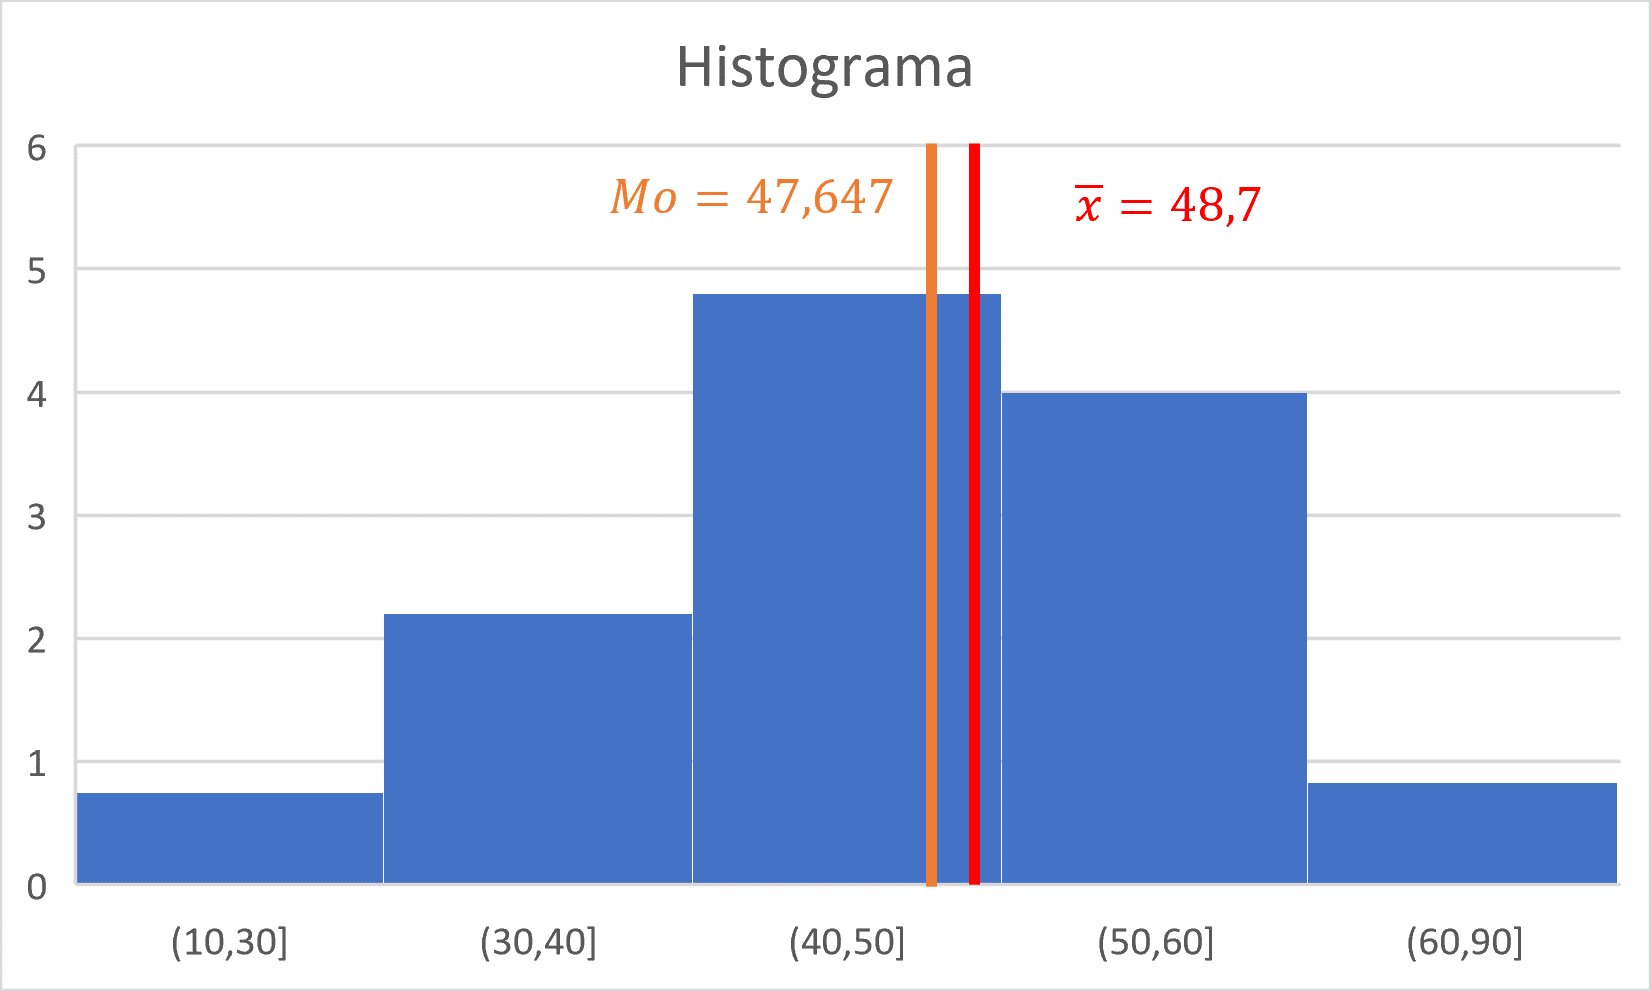
\includegraphics[width=0.8\linewidth]{Imagenes/Ej10.Simetria.png}
                \caption{Histograma mostrando la media aritmética y la moda.}
                \label{fig:Ej10.Simetria}
            \end{figure}

            \item \underline{Coeficientes de Curtosis}:\\
            Para el coeficiente de curtosis de Fischer, es necesario calcular $\mu_4$:
            $$\mu_4 = \frac{1}{n}\sum_{i=1}^5n_i(x_i-\bar{x})^4 = 153232.455$$
            $$\gamma_2(X) = \frac{\mu_4}{\sigma^4} -3 = 2.6571-3 = -0.3428 < 0$$
            
            Para el coeficiente de curtosis de Kelley, es necesario calcular $D_9$ y $D_1$:
            $$D_{9} = 60 + \frac{135-125}{25}\cdot 30 = 72
            \qquad \qquad
            D_{1} = 30 = e_1,\text{ ya que } n_1 = \frac{n}{9}=15$$
            $$K=\frac{1}{2}\frac{Q_3-Q_1}{D_9-D_1}-0.263 =
            \frac{1}{2}\frac{16.775}{42}-0.263 = -0.0632 < 0$$
            Como los coeficientes de curtosis son negativos, eso implica que la distribución es platicúrtica. Es decir, que los intervalos más centrales no sobresalen demasiado de la curva normal con la misma media aritmética y desviación típica. Además, las colas (intervalos $I_1$ e $I_5$) se encuentran por encima de esta distribución normal, como se aprecia bien en la figura \ref{fig:Ej10.Curtosis}.
            \begin{figure}[H]
                \centering
                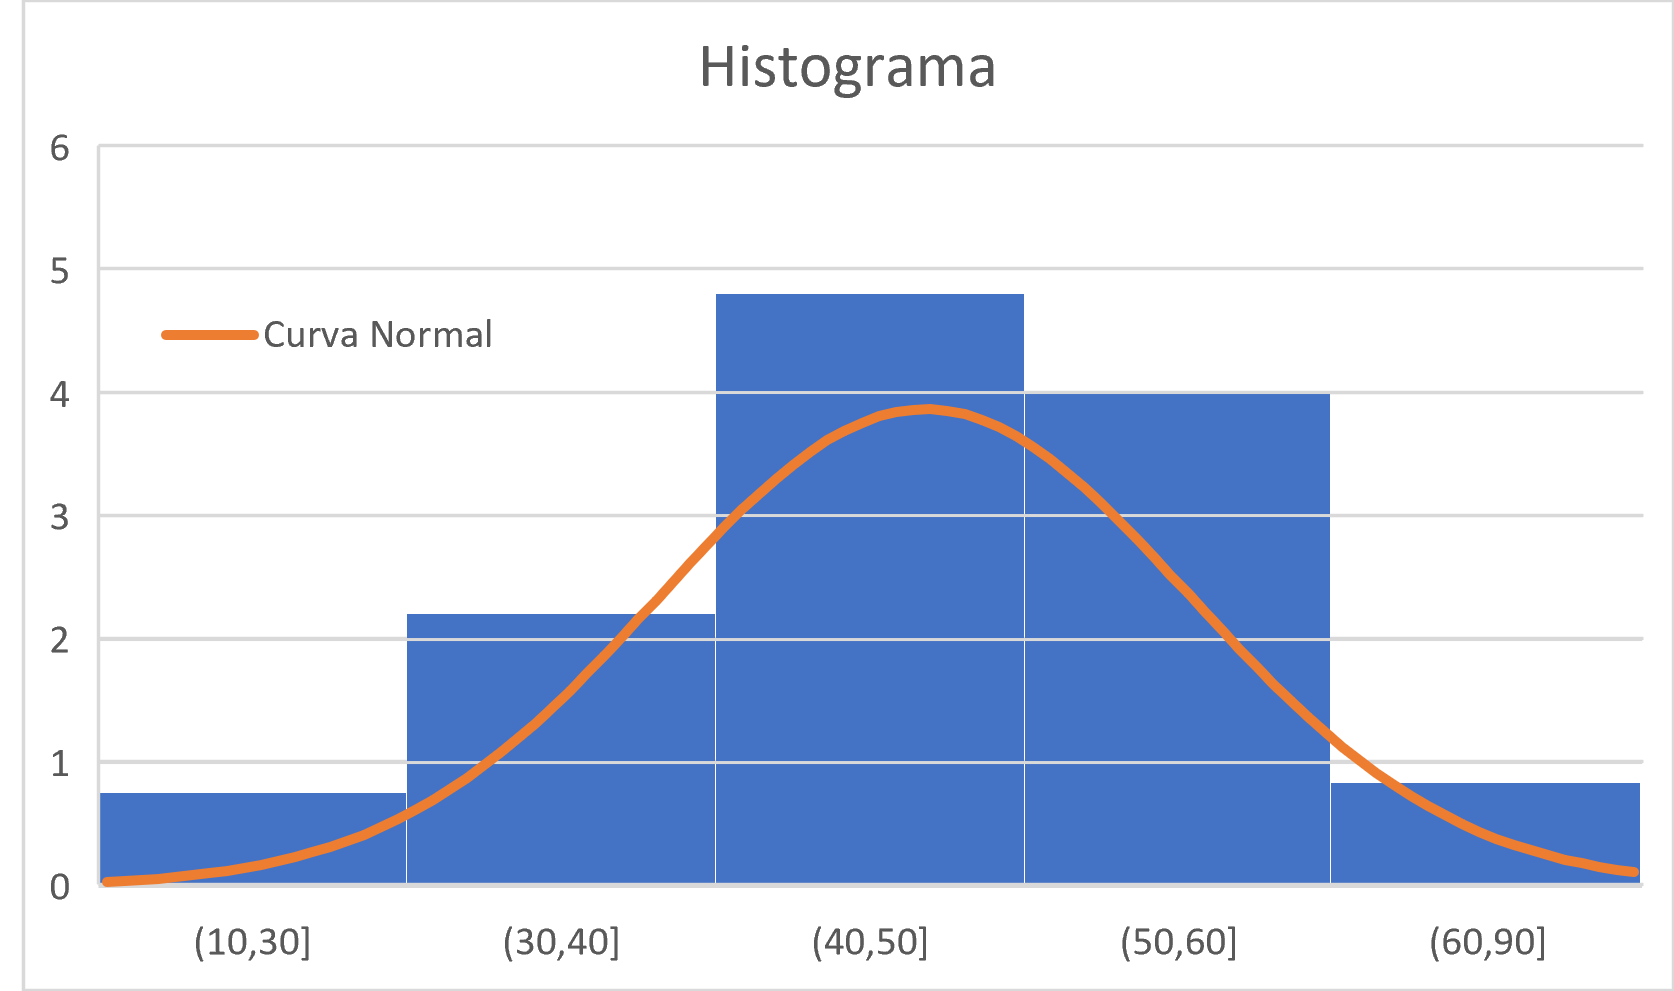
\includegraphics[width=0.8\linewidth]{Imagenes/Ej10.Curtosis.png}
                \caption{Histograma frente a la distribución normal.}
                \label{fig:Ej10.Curtosis}
            \end{figure}
        \end{itemize}
    \end{enumerate}
\end{ejercicio}
